Konzepte des zugrundeliegenden (Anwendungs)-Modells

Parallelisierungsschema (Kommunikationsmuster, Verteilung der Daten \&
Aufgaben)

Es sollte mit MPI parallelisiert werden (optional: Shared-Memory
Parallelisierung mit Threads oder OpenMP).

Leistungsanalyse des sequentiellen Codes (Verhält sich dieser
Erwartungskonform)

Skalierungsverhalten der parallelen Version

Speedup-Diagramme

Potentiell Analyse mit Vampir/Sunshot

Durchführung einer Optimierung der parallelen Version
(Kommunikationsschema etc.)

\begin{center}\rule{3in}{0.4pt}\end{center}

\section{Parallelisierungsschema}\label{parallelisierungsschema}

Das Feld wird implementiert durch ein 2D-Array of struct Ideas.

\begin{verbatim}
#define malloc_idea_matrix(name)                              \
    Idea **name = (Idea **)malloc(num_rows * sizeof(Idea *)); \
    for (int i = 0; i < num_rows; ++i)                        \
        name[i] = (Idea *)malloc(num_cols * sizeof(Idea));    \
\end{verbatim}

Es werden \emph{zwei} Felder erstellt:

\begin{verbatim}
malloc_idea_matrix(field)
malloc_idea_matrix(field_new)
\end{verbatim}

\texttt{field} wird daraufhin mit leeren Ideen initialisiert und an
zufaelligen Positionen mit Ideen bespawned. Der Inhalt von
\texttt{field} wird dann in \texttt{field\_new} kopiert. Man braucht
zwei Felder, damit eine Idee nur ein mal pro Runde ziehen kann: es wird
über den Inhalt von \texttt{field} iteriert, die gezogenen Ideen werden
in \texttt{field\_new} reingeschrieben. Wenn dannzum Beispiel eine Idee
nach rechts zieht, wird sie im naechsten Iterationsschritt nicht noch
einmal zum Zuge kommen. Kopieren ist folgendermaßen implementiert:

\begin{verbatim}
#define copy_field_into_field_new()        \
    for_every(i, num_rows, {               \
        for_every(j, num_cols, {           \
            field_new[i][j] = field[i][j]; \
          });                              \
    });
\end{verbatim}

Wir haben hier erst versucht, mittels \texttt{memcpy} das ganze
effizienter zu gestalten, nur um irgendwann festzustellen, dass das mit
derartigen 2D-Arrays nicht funktioniert, da ja bei memcpy nur die
Pointer, die auf eine row des Arrays verweisen, kopiert werden, was wir
nicht wollen, da die Ideen by value kopiert werden müssen.

Die Aufteilung dieses Feldes auf die MPI-Prozesse funktioniert nun per
horizontaler Spaltung des Feldes. Das hat den Vorteil, dass nur an zwei
Kanten kommuniziert werden muss, oben und unten. An den Raendern gibt es
``ghost rows'': Nach unten hin betrachtet wird die letzte ``reale'' row
die ``ghost row'' des naechsten ranks, und wird in dessen Feld als
zusaetzliche Reihe über dessen erster ``real row'' repraesentiert. Die
Kommunikation besteht also im Austauschen der eigenen real und ghost
rows mit den drunter und drüber liegenden Nachbarn.

\begin{figure}[htbp]
\centering
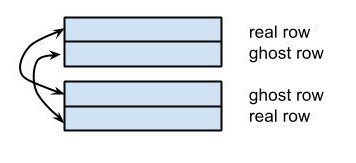
\includegraphics{pics/real-ghost-rows.jpg}
\end{figure}

Dies ermöglicht, dass jeder Prozess seine Züge unabhaengig von den
anderen Prozessen machen kann: wenn eine Idee auf einer ``real row''
nach oben respektive unten zieht, so hat sie die Informationen, was sich
in der Zielzelle, die ja eigentlich vom benachbarten Prozess bearbeitet
wird, befindet.

Aus dem Vorhandensein dieser zwei rows, die an den Raendern der
rank-spezifischen fields jeweils sind, folgt das Konzept von
``independent'' und ``dependent'' rows:

\begin{figure}[htbp]
\centering
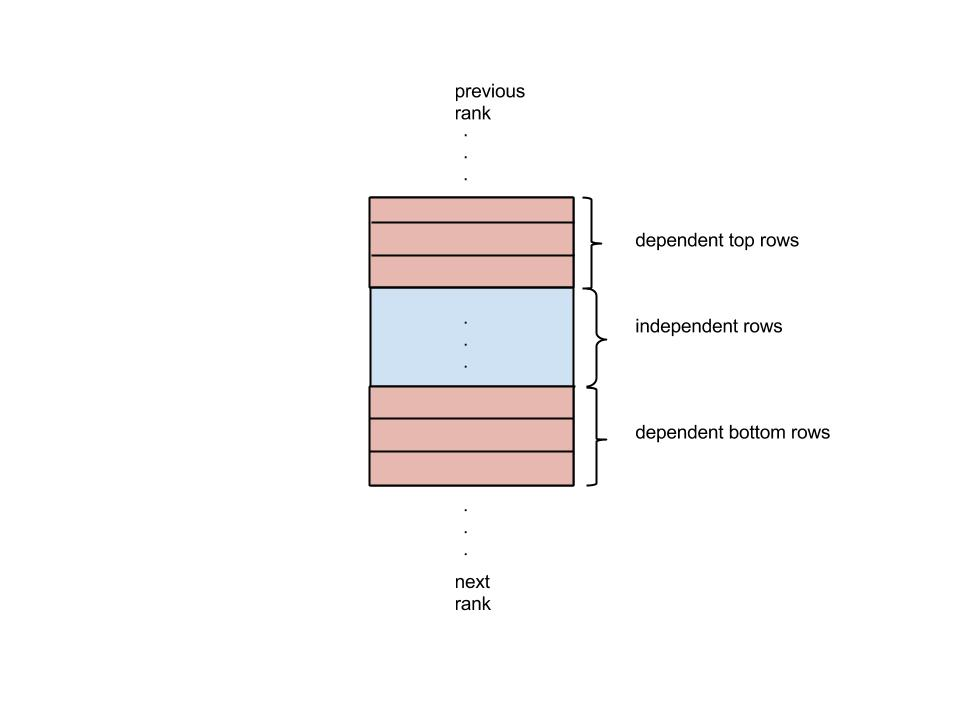
\includegraphics{pics/dependent-rows.jpg}
\end{figure}

\emph{Drei} rows sind an den Raendern jeweils ``dependent'': die zwei
aeussersten müssen direkt mit den Nachbarn kommunizieren und
drittaeusserste kann durch Bewegung von Ideen in die zweitaeusserste row
ebenso ``dependent'' sein. ``Dependent'' heisst hier: die Bewegung von
Ideen kann die anliegenden ranks ``etwas angehen''. Die ``independent''
rows hingegen tangieren die anderen ranks nicht, jedenfalls nicht
innerhalb \emph{einer Runde}, denn pro Runde kann eine Idee ja nur ein
Feld weiter ziehen. Aus dieser Erkenntnis folgt, dass die Bewegung im
Feldabschnitt der ``independent rows'' unabhaengig von den andern ranks
erfolgt, die der ``dependent rows'' allerdings nicht und somit zeitlich
orchestriert werden muss.

Diese Orchestration erfolgt in drei Schritten, die Schritte gelten für
jeden rank:

\begin{enumerate}
\def\labelenumi{\arabic{enumi}.}
\itemsep1pt\parskip0pt\parsep0pt
\item
  Bewege die Ideen die sich auf den ``independent rows'' befinden.
\item
  Bewege die Ideen, die sich auf den ``dependent top rows'' befinden.

  \begin{enumerate}
  \def\labelenumii{\arabic{enumii}.}
  \itemsep1pt\parskip0pt\parsep0pt
  \item
    Sende top real und top ghost row zu oberem Nachbarn.
  \item
    Empfange top real und top ghost row von unterem Nachbarn.
  \end{enumerate}
\item
  Analog wie 2. für die bottom dependent rows.
\end{enumerate}

Das Senden und Empfangen wird mittels \texttt{MPI\_Isend} und
\texttt{Irecv} realisiert. Dies hat den Vorteil, dass real und ghost row
nacheinander versendet werden, ohne erst auf die Empfangsbestaetigung
für das erste Paket zu warten.

Im Code sieht das so aus:

\begin{verbatim}
#define send_ideas(ideas_arr, to, tag, req) \
  MPI_Isend(ideas_arr, num_cols, mpi_idea_type, to, tag, MPI_COMM_WORLD, &req) 

#define receive_ideas_into(ideas_arr, from, tag, req) \
  MPI_Irecv(ideas_arr, num_cols, mpi_idea_type, from, tag, MPI_COMM_WORLD, &req) 

#define send_top_rows(field) \
  /* send our first ghost row into the bottom real row of the previous rank */ \
  send_ideas(field[0], prev_rank, GHOST, req);                                \
  /* send our first real row into the bottom ghost row of the previous rank */ \
  send_ideas(field[1], prev_rank, REAL, req2);                                 \

#define receive_into_bottom_rows(field) \
  /* receive first ghost row from next rank into our bottom real row */ \
  receive_ideas_into(field[num_rows-2], next_rank, GHOST, req);        \
  /* receive first real row from next rank into our bottom ghost row */ \
  receive_ideas_into(field[num_rows-1], next_rank, REAL, req2);         \
\end{verbatim}

Der \texttt{mpi\_idea\_type} wird hierbei auf folgende (kompliziert
anzuschauende) Art definiert:

\begin{verbatim}
#define mpi_define_idea_type()                                               \
  int          blocklengths[5] = {1,1,1,1,1};                                  \
  MPI_Datatype types[5] = {MPI_INT,MPI_INT,MPI_INT, MPI_INT, MPI_INT};       \
  MPI_Datatype mpi_idea_type;                                                \
  MPI_Aint     offsets[5];                                                   \
  offsets[0] = offsetof(Idea, a);                                            \
  offsets[1] = offsetof(Idea, b);                                            \
  offsets[2] = offsetof(Idea, c);                                            \
  offsets[3] = offsetof(Idea, h);                                            \
  offsets[4] = offsetof(Idea, empty);                                        \
    MPI_Type_create_struct(5, blocklengths, offsets, types, &mpi_idea_type); \
    MPI_Type_commit(&mpi_idea_type);                                         \
\end{verbatim}

Die Kommunikation benutzt im Übrigen \texttt{field\_new} zum Austausch
der Daten; am Ende einer Runde wird dieses dann pro Prozess in
\texttt{field} kopiert.

Es ist entscheidend, die einzelnen Schritte per \texttt{MPI\_Barrier}
abzutrennen, da es sonst zu race conditions kommt.

\section{Implementation der
Visualisierung}\label{implementation-der-visualisierung}

Wir haben die Visualisierung lokal mit Pygame implementiert. Die Daten
werden von C, sofern \texttt{\#define DRAW} gilt, per Prozess per Runde
in \texttt{src/draw/out/\$round-\$proc} exportiert und dann im
Nachhinein von Python eingelesen. Dies hat den entscheidenden Nachteil,
dass zum einen der Nutzen des Clusters eingeschraenkt ist: um diesen zu
nutzen \emph{und} die Visualisierung zu nutzen, müssen die Output-Files
auf dem Cluster generiert und dann nach local kopiert werden (das haben
wir auch implementiert per einem automatisierten Deploy script, dass den
Quellcode auf den cluster rsynct, dort das Programm laufen laesst und
dann die Output-Files wieder per rsync zurück kopiert; dies ist bloß
leider sehr eingeschraenkt praktikabel wegen der Dateimenge - damit wird
der Performance-Gewinn durch das Mehr an Prozessen unterminiert). Zum
anderen ist von Nachteil, dass hiermit keine Realtime-Visualisierung
möglich ist.

Das Problem von Realtime-Visualisierung scheint uns aber kein triviales
zu sein: schließlich müssten die Daten vermutlich in einem master rank
pro Runde gesammelt werden um sie dann grafisch auszugeben; außerdem war
uns nicht ganz klar, wie und ob so etwas überhaupt auf dem Cluster - per
X-Forwarding - funktionieren würde, weshalb wir uns dann für die lokale
Scripting-Variante entschieden haben.

\section{Performance}\label{performance}

Wie zu erwarten, ist die Performance mit aktiviertem IO ca. um den
Faktor 80 schlechter als ohne:

\begin{figure}[htbp]
\centering
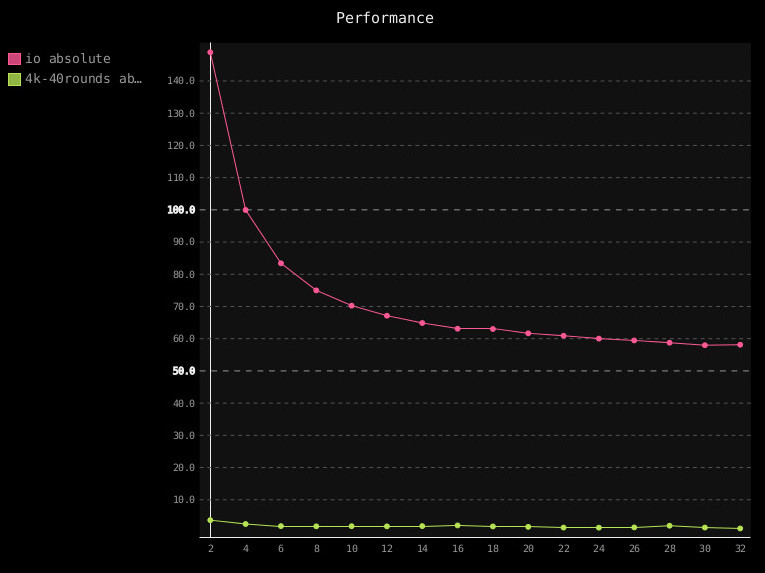
\includegraphics{pics/io-vs-no-io absolute.jpg}
\end{figure}

Hingegen ist der Speedup aehnlich (ein Wert von 1 hieße eine lineare
Relation zwischen Anzahl von Prozessen und absoluter Geschwindigkeit,
weniger entsprechend weniger effektiv):

\begin{figure}[htbp]
\centering
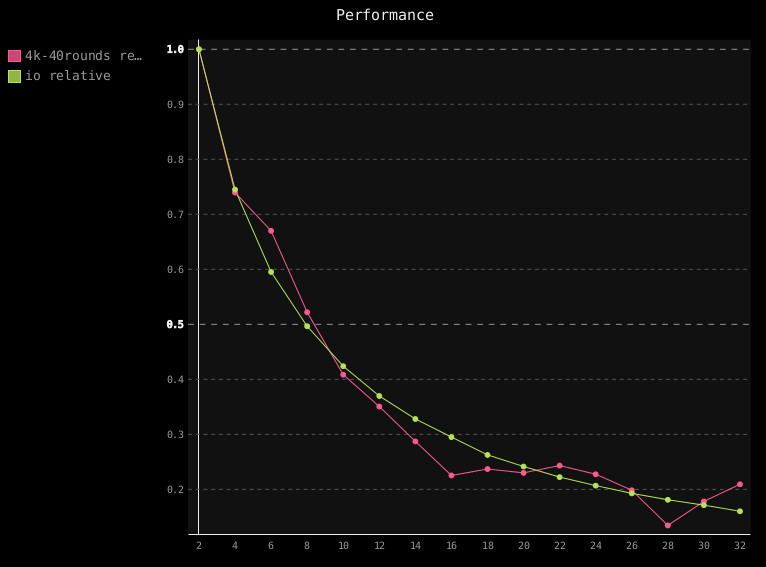
\includegraphics{pics/io-vs-no-io rel.jpg}
\end{figure}

Der absolute Verlauf ohne IO sieht wie folgt aus:

\begin{figure}[htbp]
\centering
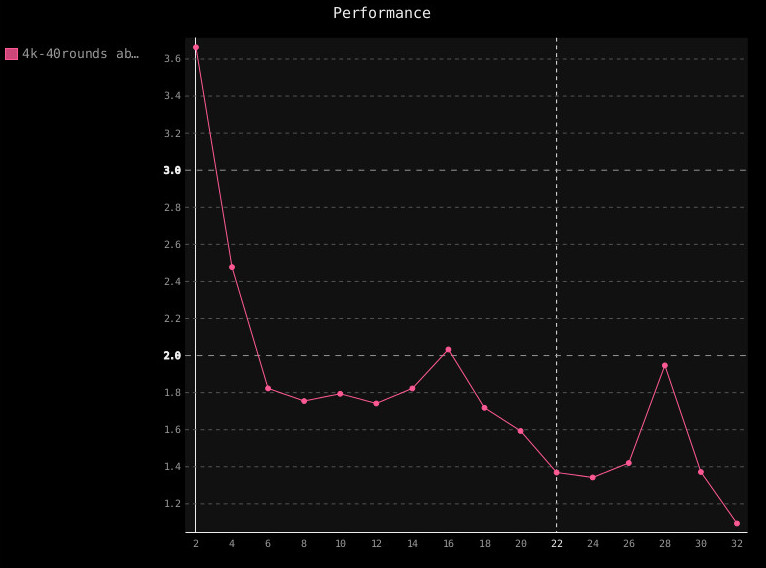
\includegraphics{pics/perf-abs.jpg}
\end{figure}

Die Ausschlaege sind in diesem Fall relativ stark, sie treten allerdings
immer auf und treten dann auf, wenn ein zusaetzlicher Rechner innerhalb
des Clusters dazukommt, da dann ein Mehraufwand an Network-Kommunikation
auftritt.

Die relativen Speedups und die Abnahme der Effizienz ist damit zu
erklaeren, dass das Verhaeltnis von MPI-Kommunikation zu realer
Rechenzeit steigt und insofern der Anteil an ``teuren'' Instruktionen
staendig größer wird.

\section{Optimierung}\label{optimierung}

Folgende Optimierungen haben wir im Laufe der Entwicklung vorgenommen:

\begin{enumerate}
\def\labelenumi{\arabic{enumi}.}
\itemsep1pt\parskip0pt\parsep0pt
\item
  \texttt{MPI\_Isend/Recv} anstelle von \texttt{Send/Recv} einsetzen.
  Dies brachte ca. 10\% Speedup.
\item
  Den \texttt{field\_new} -\textgreater{} \texttt{field} Kopiervorgang
  nur einmal ausführen. Dies war Bestandteil eines tieferen Problems,
  was uns viele Stunden Bugs und Mühen beschaeftigt hat, auch wenn es im
  Nachhinein trivial wirkt: die ersten Wochen hatten wir das
  \texttt{field} (und nicht \texttt{field\_new} in der MPI-Kommunikation
  verschickt. Dies führte zu Korruptionen im Feld, die Ideen vermehrten
  sich, aber nur manchmal, bei einer genügend hohen Ideendichte. Durch
  die Zufaelligkeit der Simulation war das ganze auch quasi unmöglich zu
  debuggen; der Schleier wurde erst von unseren Augen genommen, als wir
  eine Drop-In ``quasi-unit-test'' Bewegungsmethode implementierten, die
  die Ideen immer nur nach unten gehen ließ. Es handelt sich insofern
  nicht um eine Performance-Optimierung, sondern um eine Optimierung der
  Zuverlaessigkeit des Systems.
\item
  Den schon oben angesprochenen Versuch, das Kopieren von
  \texttt{field\_new} in \texttt{field} per \texttt{memcpy} umzusetzen.
  Auch dies funktionierte leider erstmal ``irgendwie'', sodass der
  Eindruck entstand, die Simulation tue das, was sie tuen solle. Leider
  wurden auf diese Art ja aber nur Pointer auf die einzelnen rows
  kopiert, was zu fiesen, ebenso schwer zu findenden Bugs führte.
  Natürlich haette es enorm geholfen, sich einfach besser mit C
  auszukennen; so war man auf das kollektive Wissen von Stack Overflow
  angewiesen und verlor viele Stunden mit Bugsuche.
\end{enumerate}

Generell also kann man den Entwicklungsprozess, was den MPI-Part anging,
hauptsaechlich als ein Suchen nach Bugs, die den Großteil der Zeit
extrem ``mysteriöse'' Resultate erzeugten, beschreiben. Leider war
Debug-Tooling hier nicht wirklich hilfreich, zum einen wegen der
involvierten Randomness, die zu nicht reproduzierbaren Ergebnissen
führte, zum anderen, weil erste spezifische Konstellationen des Feldes
zu korrupierten Ergebnissen führten.

Dementsprechend kann man unsere Strategie bezüglich MPI, als denn alles
so funktionierte, wie es sollte, als sehr defensiv beschreiben; das
System erschien uns so fragil, und wir wollten endlich eine
funktionierende Basis für die Simulation an sich haben. Daher kann es
durchaus sein, dass der MPI-Part noch optimiert werden könnte.

Dazu kam, dass die Visualisierung eh am besten aussah mit einem Feld von
200x200 Ideen. Diese Größe konnte man problemlos auch lokal in einigen
Sekunden mit MPI generieren. Außerdem war wie schon erwaehnt in der
Variante mit auf dem Cluster rechnen, Daten nach local kopieren und dort
visualisieren das Bottleneck nicht MPI oder C überhaupt, sondern rsync.

Wenn man also weiter haette optimieren wollen, dann vermutlich in erster
Linie an der Toolchain an sich - eine Visualisierung ohne I/O auf dem
Cluster waere hier mit Abstand der gewinnbringendste Approach.

Wir haben den Fokus dann eher auf das Ausbauen der Simulationslogik und
der Darstellung dieser gelegt, da wie gesagt der Stand der Dinge
hinsichtlich der Engine ausreichend war, um für die Visualisierung
geeignete Feldgrößen mit einer ausreichenden Anzahl an Runden
hinreichend schnell zu berechnen.
